%%% lorem.tex --- 
%% 
%% Filename: lorem.tex
%% Description: 
%% Author: Ola Leifler
%% Maintainer: 
%% Created: Wed Nov 10 09:59:23 2010 (CET)
%% Version: $Id$
%% Version: 
%% Last-Updated: Wed Nov 10 09:59:47 2010 (CET)
%%           By: Ola Leifler
%%     Update #: 2
%% URL: 
%% Keywords: 
%% Compatibility: 
%% 
%%%%%%%%%%%%%%%%%%%%%%%%%%%%%%%%%%%%%%%%%%%%%%%%%%%%%%%%%%%%%%%%%%%%%%
%% 
%%% Commentary: 
%% 
%% 
%% 
%%%%%%%%%%%%%%%%%%%%%%%%%%%%%%%%%%%%%%%%%%%%%%%%%%%%%%%%%%%%%%%%%%%%%%
%% 
%%% Change log:
%% 
%% 
%% RCS $Log$
%%%%%%%%%%%%%%%%%%%%%%%%%%%%%%%%%%%%%%%%%%%%%%%%%%%%%%%%%%%%%%%%%%%%%%
%% 
%%% Code:

\chapter{Results}
\label{cha:results}

This chapter is dedicated to show the analysis' results. In favor of clarity and organization, this chapter will be divided into two main sections: the first treating each gas exposure individually and the other averaging exposures of the same gas mixture. Subsections on the models used also are present. The plots presented in this section were made using \textit{ad-hoc} plotting functions.

Initially the regression analysis was done in the pre-processed data presented in Chapter~\ref{cha:data}, i.e. each observation corresponds to a gas exposure. It is important to remind the reader that in this data, each unique gas mixture was exposed (i.e. an exposure) twelve times: four frequency cycles through three experiment repetitions, yielding 1500 observations. 

An assessment of correlation between features is first conducted and shown in Figure~\ref{fig:cor-mat}.

\begin{figure}[h]
	\centering
	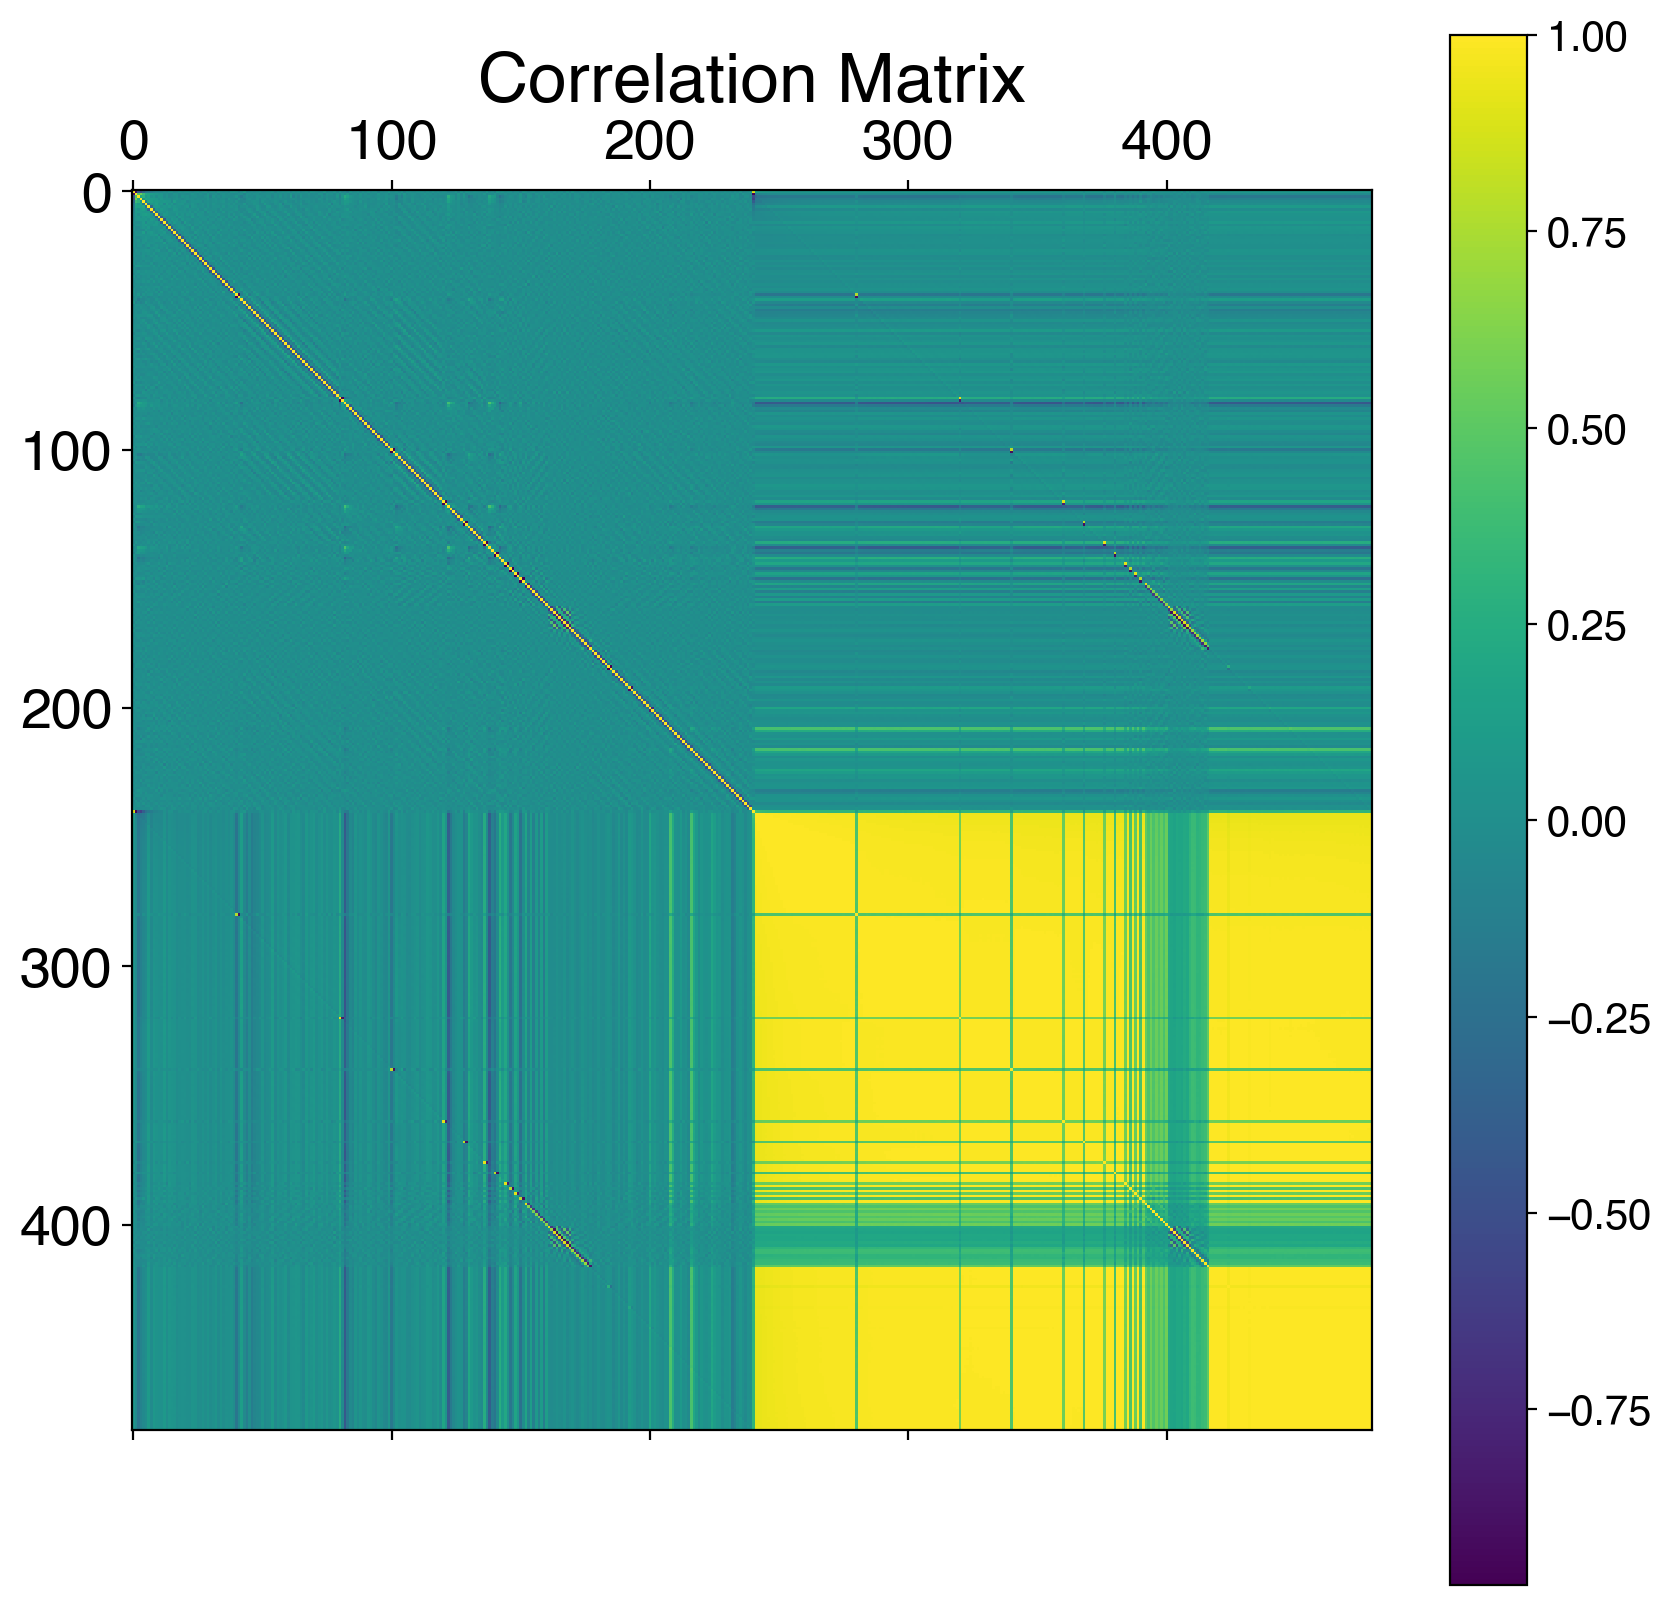
\includegraphics[width=0.7\textwidth]{../figures/correlation-matrix.png}
	\caption{Correlation matrix of features.}
	\label{fig:cor-mat}
\end{figure}

\section{Individual exposures}

\subsection{OLS}

As explained in Chapter~\ref{cha:methods}, \acrshort{ols} is treated here as a baseline. The actual vs. predicted plot in Figure~\ref{fig:ols-exposures} shows the predictions of this model.

\begin{figure}[h]
	\centering
	\includegraphics[width=1\textwidth]{../figures/ols-exposures.png}
	\caption{OLS prediction for individual exposures}
	\label{fig:ols-exposures}
\end{figure}

\subsection{PCR}
\label{subsec:pcr1}

Following the methodology of Chapter~\ref{cha:methods}, a \acrshort{pca} is conducted with two components in an attempt to visualize the data in a lower dimensional space in Figure~\ref{fig:pca}. 

\begin{figure}[!htb]
	\centering
	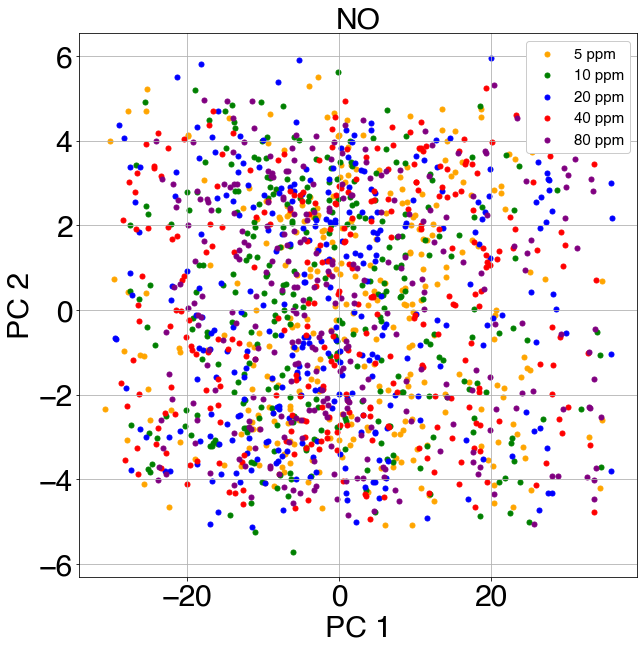
\includegraphics[width=0.30\textwidth]{../../figures/pcaNO.png}
	\hfill
	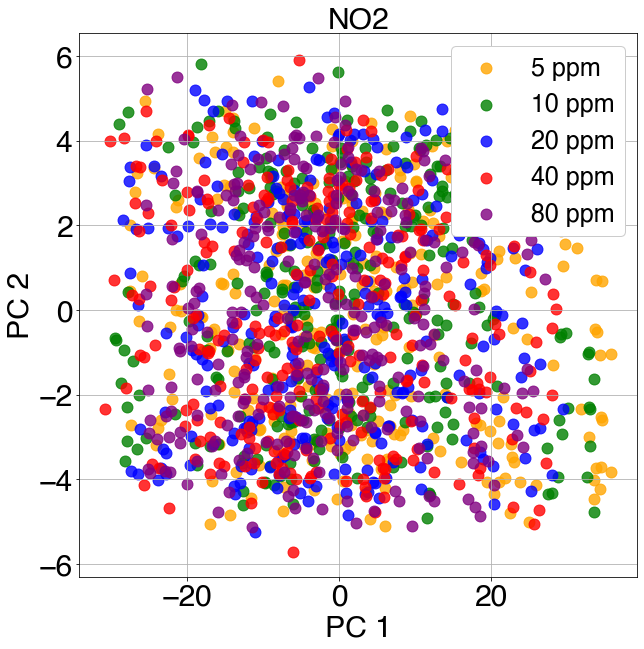
\includegraphics[width=0.30\textwidth]{../../figures/pcaNO2.png}
	\hfill
	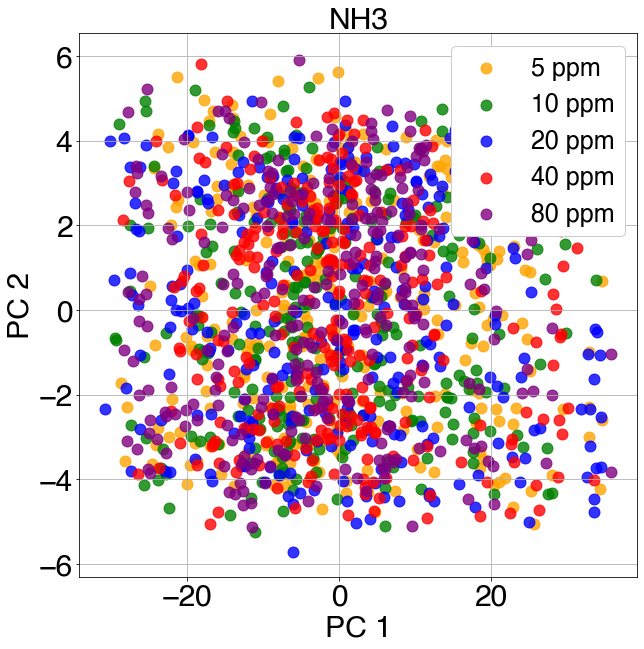
\includegraphics[width=0.30\textwidth]{../../figures/pcaNH3.png}
	\caption{\acrshort{pca} with two components for the three gases.}
	
\label{fig:pca}
\end{figure}

Furthermore, an explained variance plot is shown in Figure~\ref{fig:pcr-exp-var}. The first two \acrshort{pc}s explain approximately 40\% of the total variance, reaching 80\% around 100 components.

\begin{figure}[h]
	\centering
	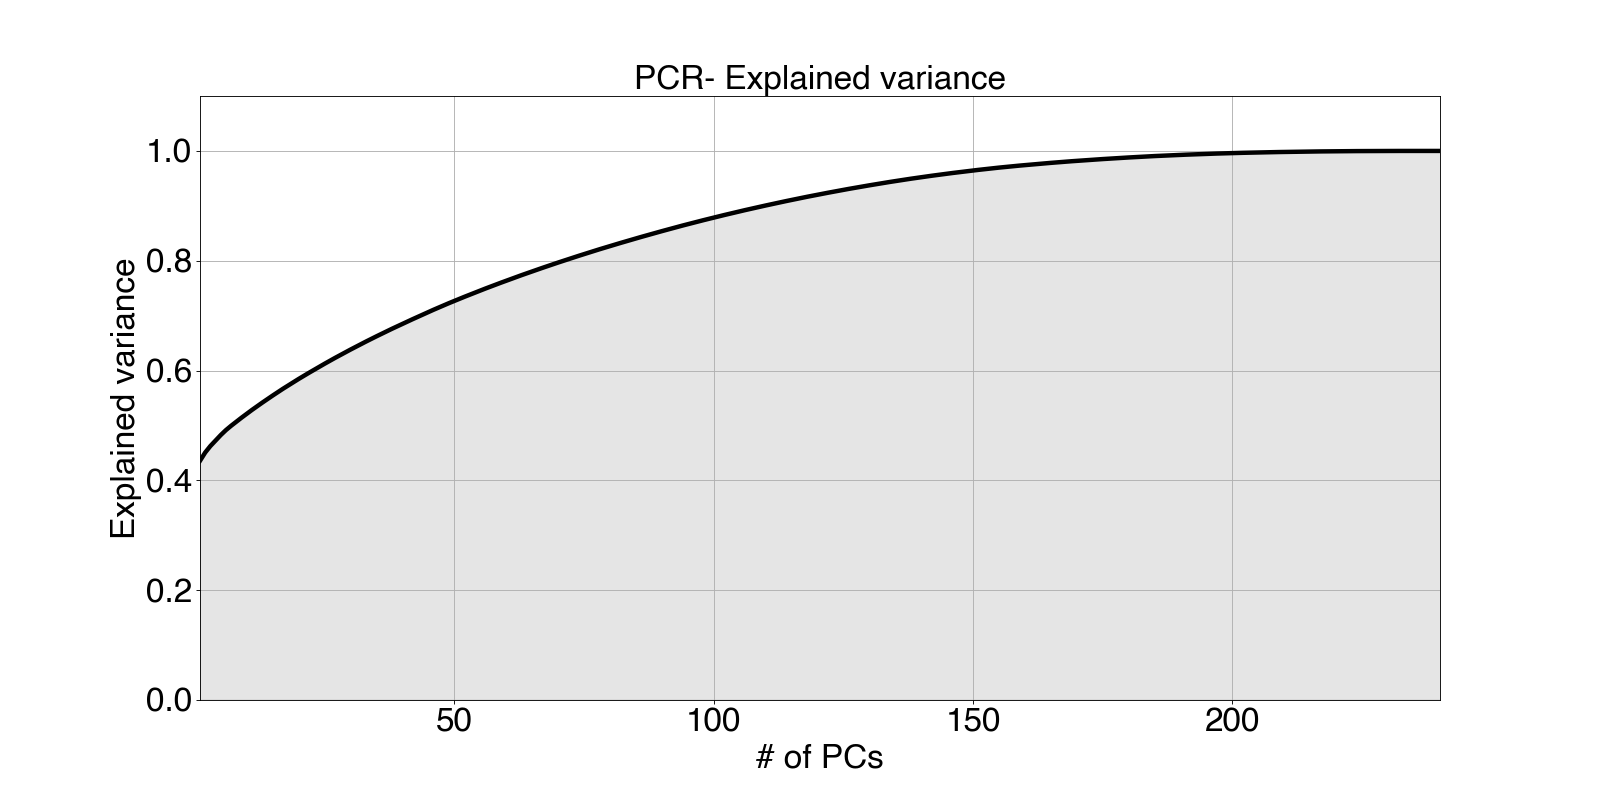
\includegraphics[width=1\textwidth]{../figures/pcr-explained-variance.png}
	\caption{Explained variance}
	\label{fig:pcr-exp-var}
\end{figure}

After this exploration of \acrshort{pca}, the analysis proceeds to fit a \acrshort{pcr} model to the data. The choice of number of \acrshort{pc}s was made via cross-validation using \acrshort{rmse} as the loss function, as can be seen in Figure~\ref{fig:pcr-cv-exposures}. Choosing only one components yields the minimum loss, around 27.

\begin{figure}[h]
	\centering
	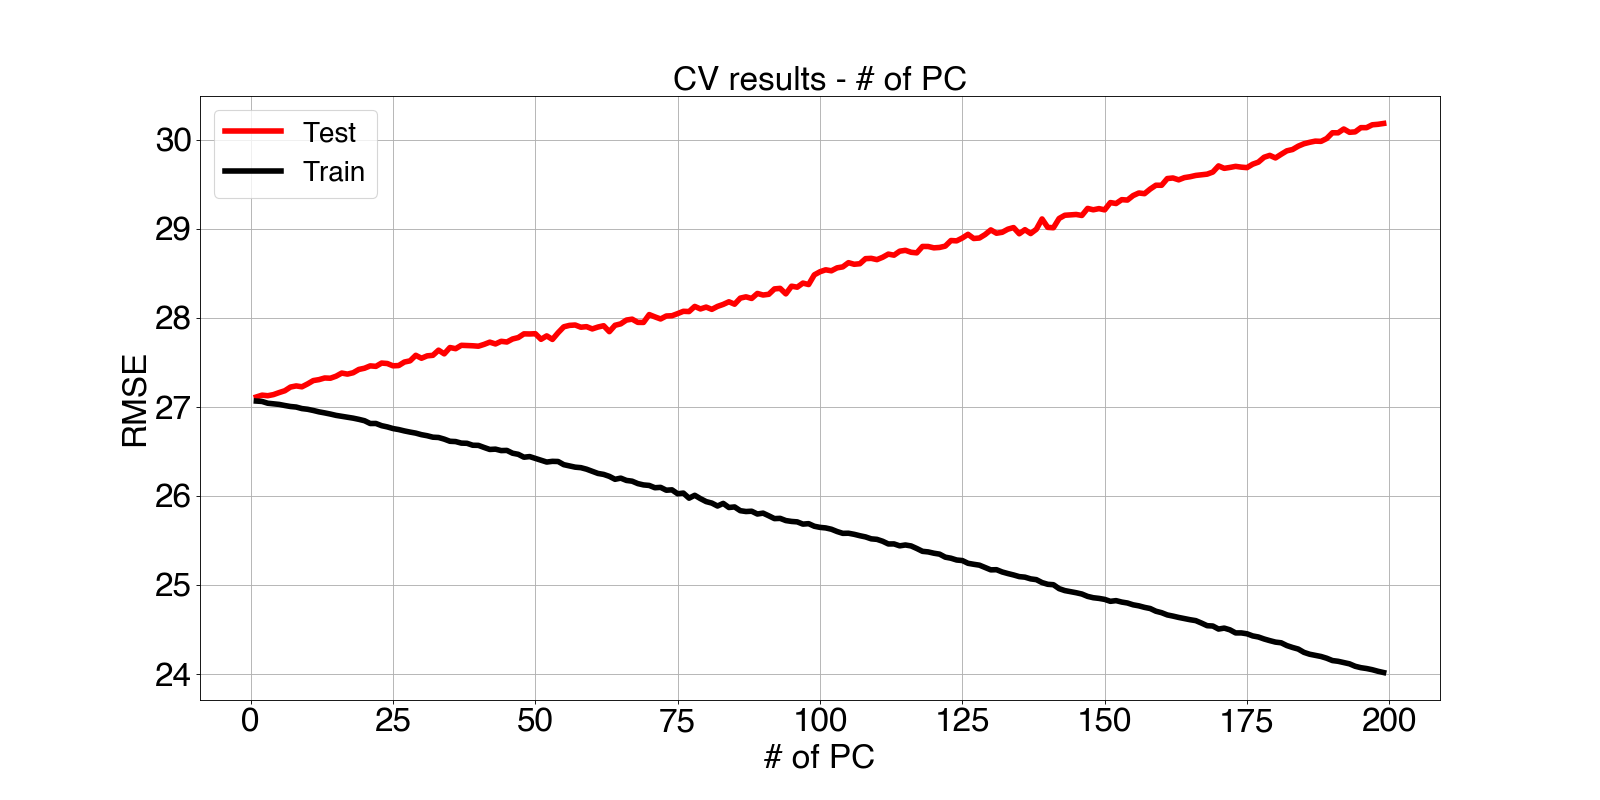
\includegraphics[width=1\textwidth]{../figures/pcr-cv-exposures.png}
	\caption{Number of \acrshort{pc}s selection via \acrshort{cv}.}
	\label{fig:pcr-cv-exposures}
\end{figure}

After the choosing the number of components, the regression line was fit to the training data and used to predict unseen validation data. A quick way to visualize and assess the quality of the fit is an actual vs. predicted plot,  shown in Figure~\ref{fig:pcr-exposures}.

\begin{figure}[h]
	\centering
	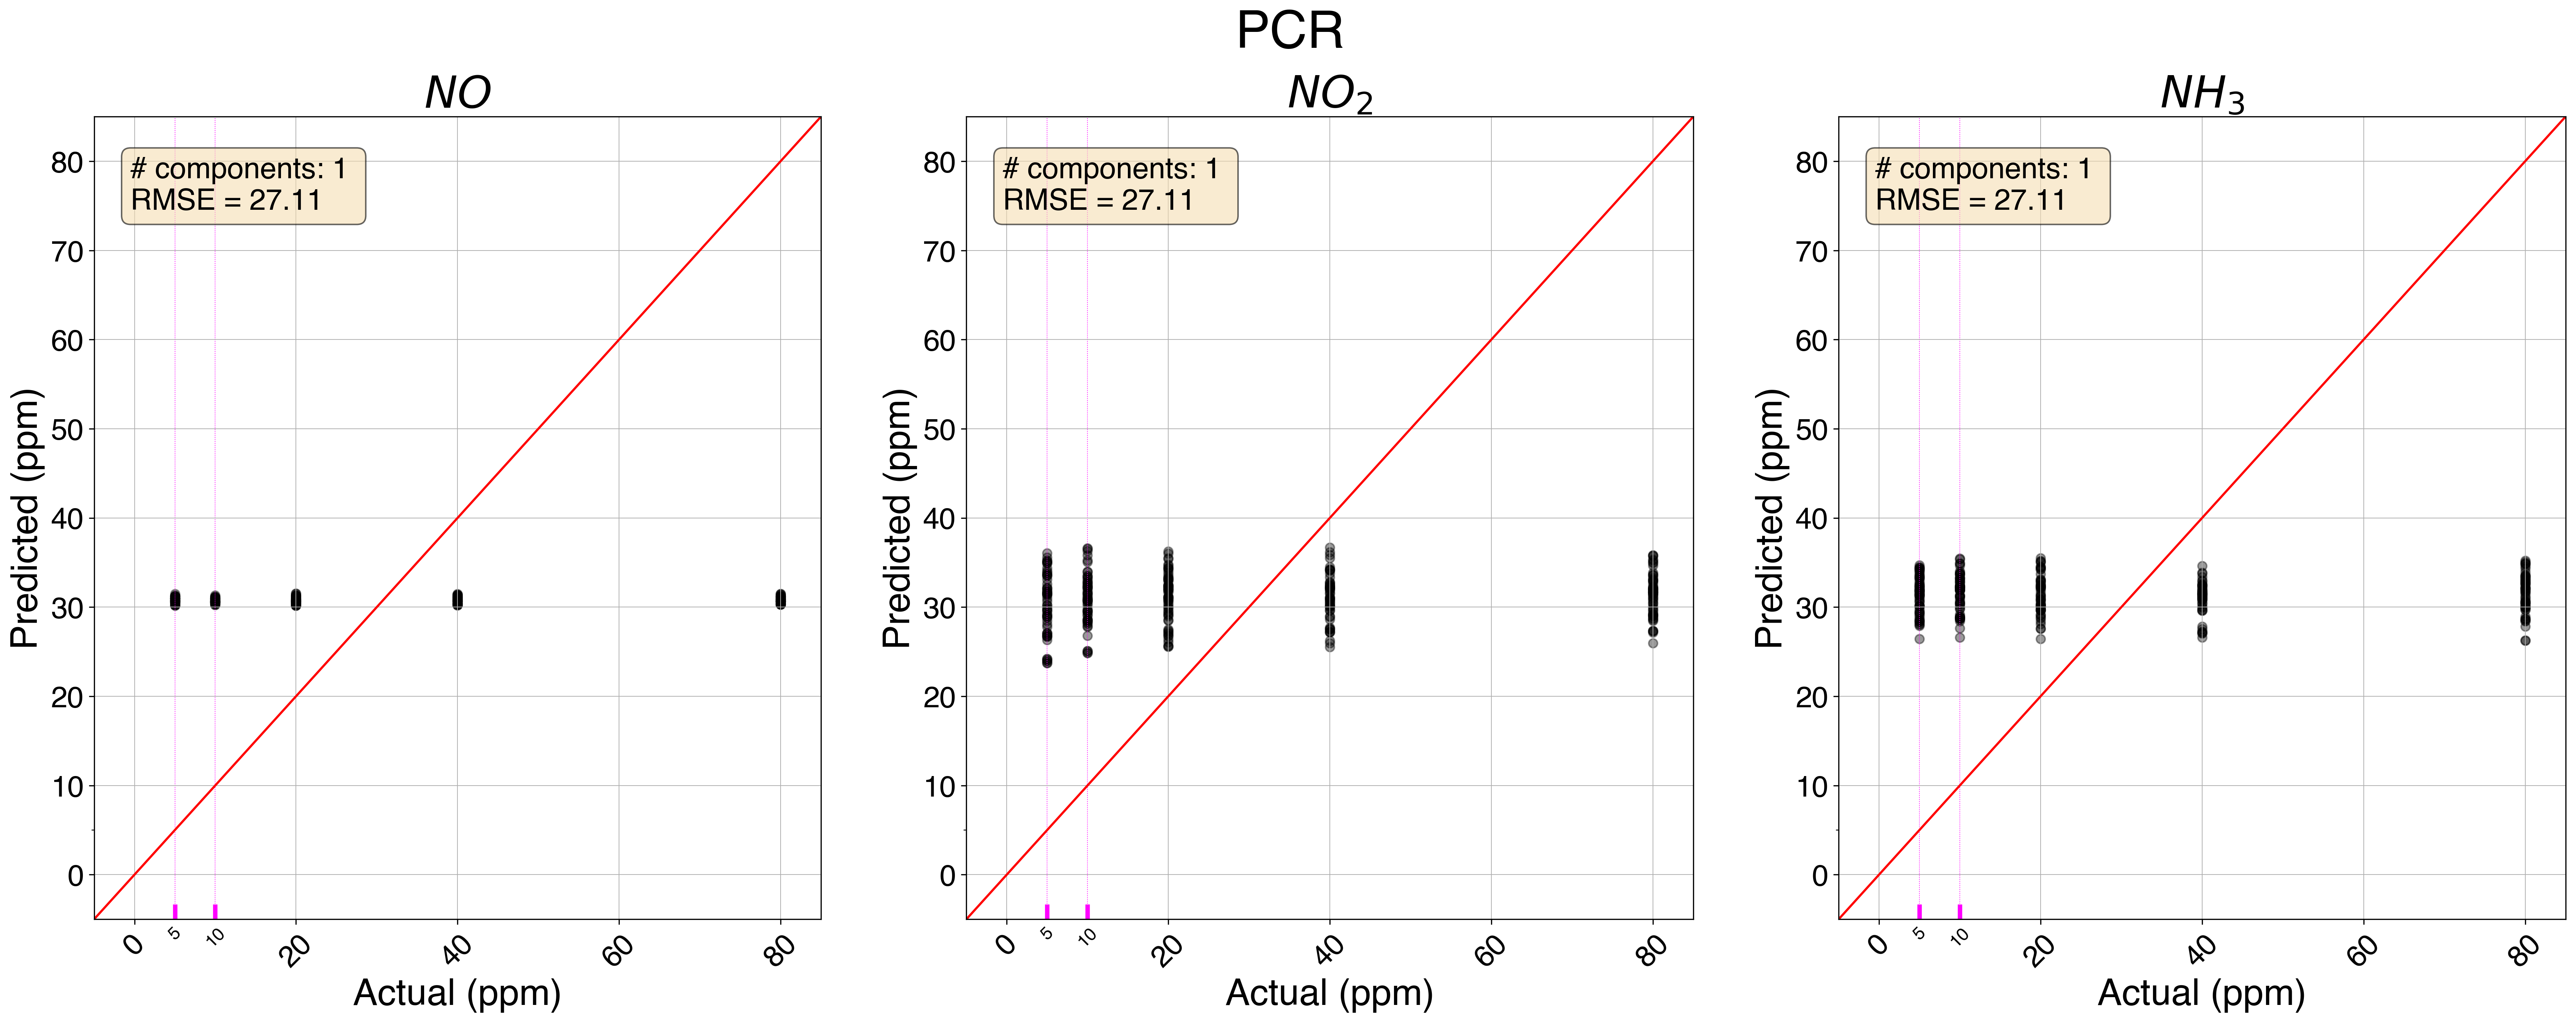
\includegraphics[width=1\textwidth]{../figures/pcr-exposures.png}
	\caption{PCR prediction for individual exposures}
	\label{fig:pcr-exposures}
\end{figure}

\newpage
\subsection{PLSR}

Following the proposed model progression, the analysis proceeds to fit the \acrshort{plsr} model. A similar pipeline to Section~\ref{subsec:pcr1} was used. First, in Figure~\ref{fig:pls}, the choice of only two \acrshort{pls} components allowed visualization of data in a two dimensional plot. Moreover, total explained variance is shown in Figure~\ref{fig:pls-exp-var}. Once again, cross-validation using \acrshort{rmse} yields a single component as the best choice, which is then used to fit and predict gas concentrations in Figure~\ref{fig:plsr-exposures}.

\begin{figure}[!htb]
	\centering
	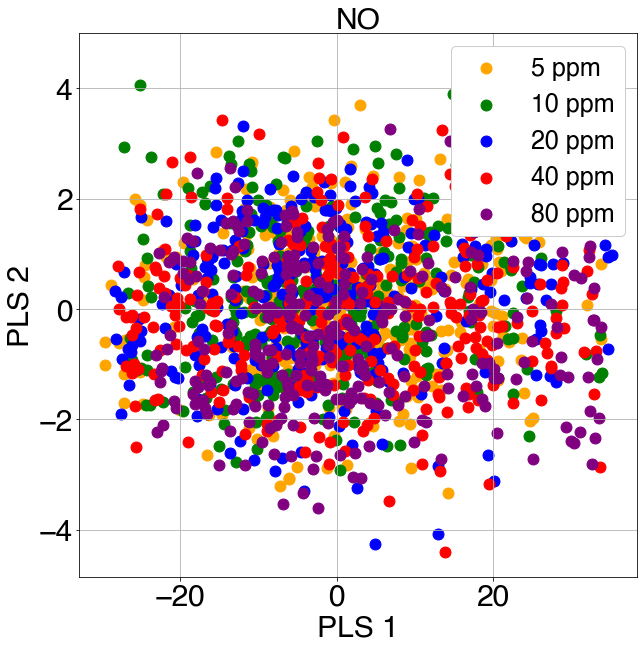
\includegraphics[width=0.32\textwidth]{../../figures/plsNO.png}
	\hfill
	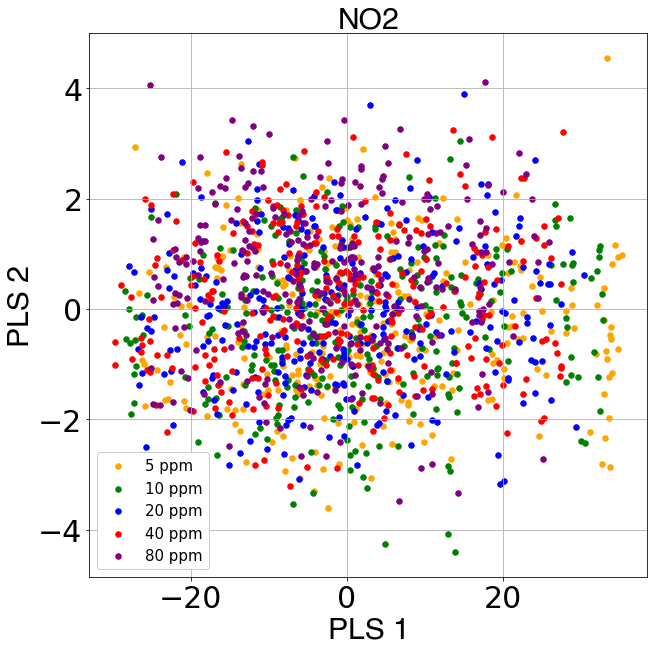
\includegraphics[width=0.32\textwidth]{../../figures/plsNO2.png}
	\hfill
	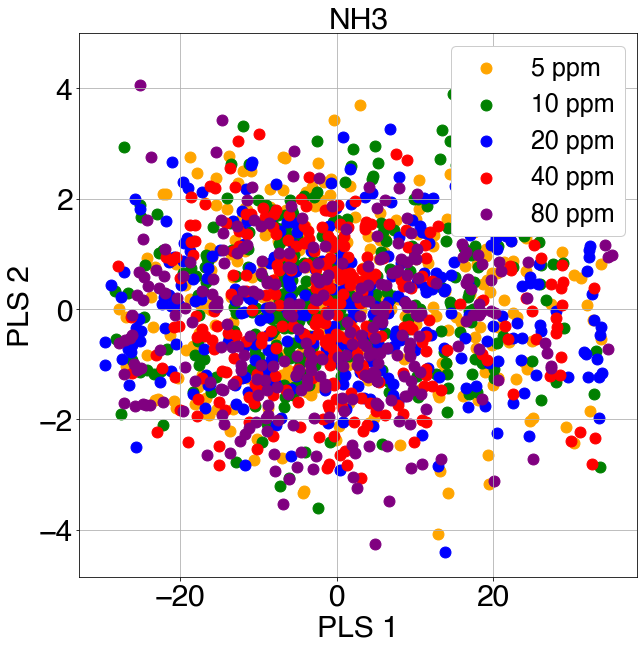
\includegraphics[width=0.32\textwidth]{../../figures/plsNH3.png}
	\caption{\acrshort{pls} with two components for the three gases.}
	\label{fig:pls}
\end{figure}

\begin{figure}[h]
	\centering
	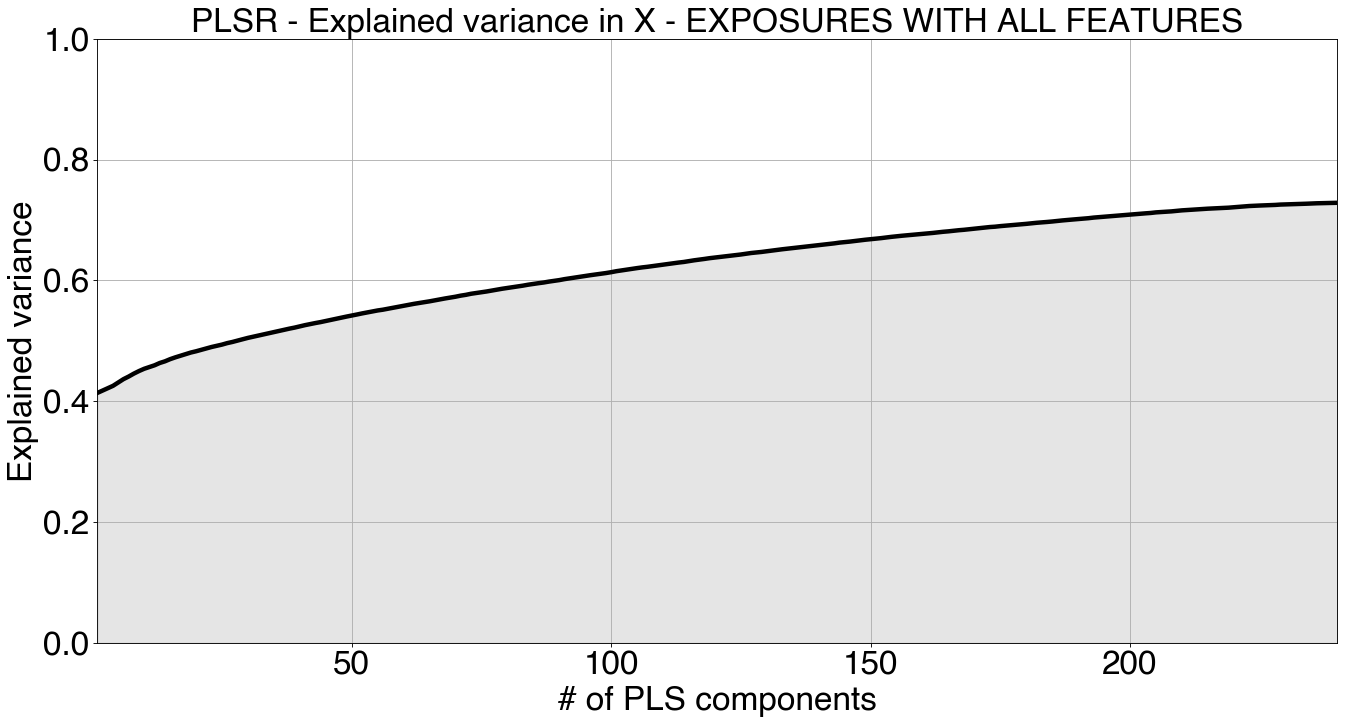
\includegraphics[width=1\textwidth]{../figures/pls-explained-variance.png}
	\caption{PLS - Explained variance of X}
	\label{fig:pls-exp-var}
\end{figure}

\begin{figure}[h]
	\centering
	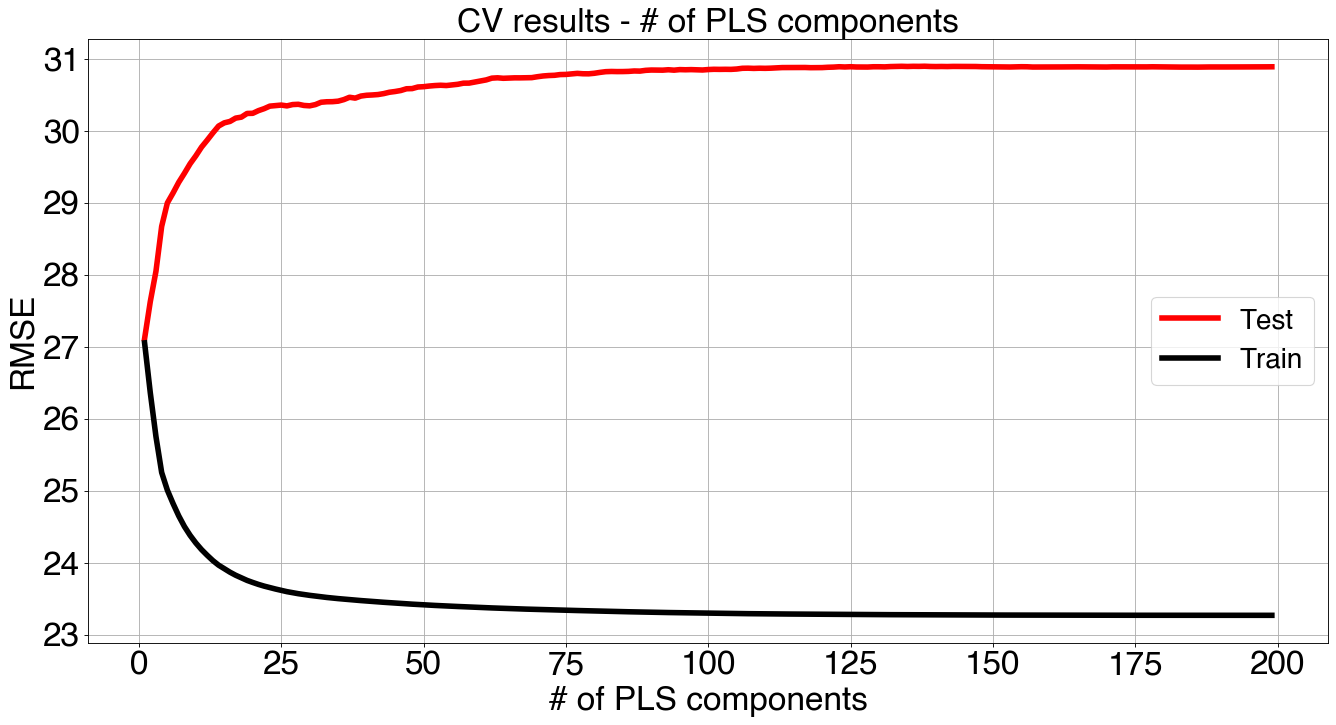
\includegraphics[width=1\textwidth]{../figures/pls-cv-exposures.png}
	\caption{Number of \acrshort{pls} components selection via \acrshort{cv}.}
	\label{fig:pls-cv-exposures}
\end{figure}

\begin{figure}[h]
	\centering
	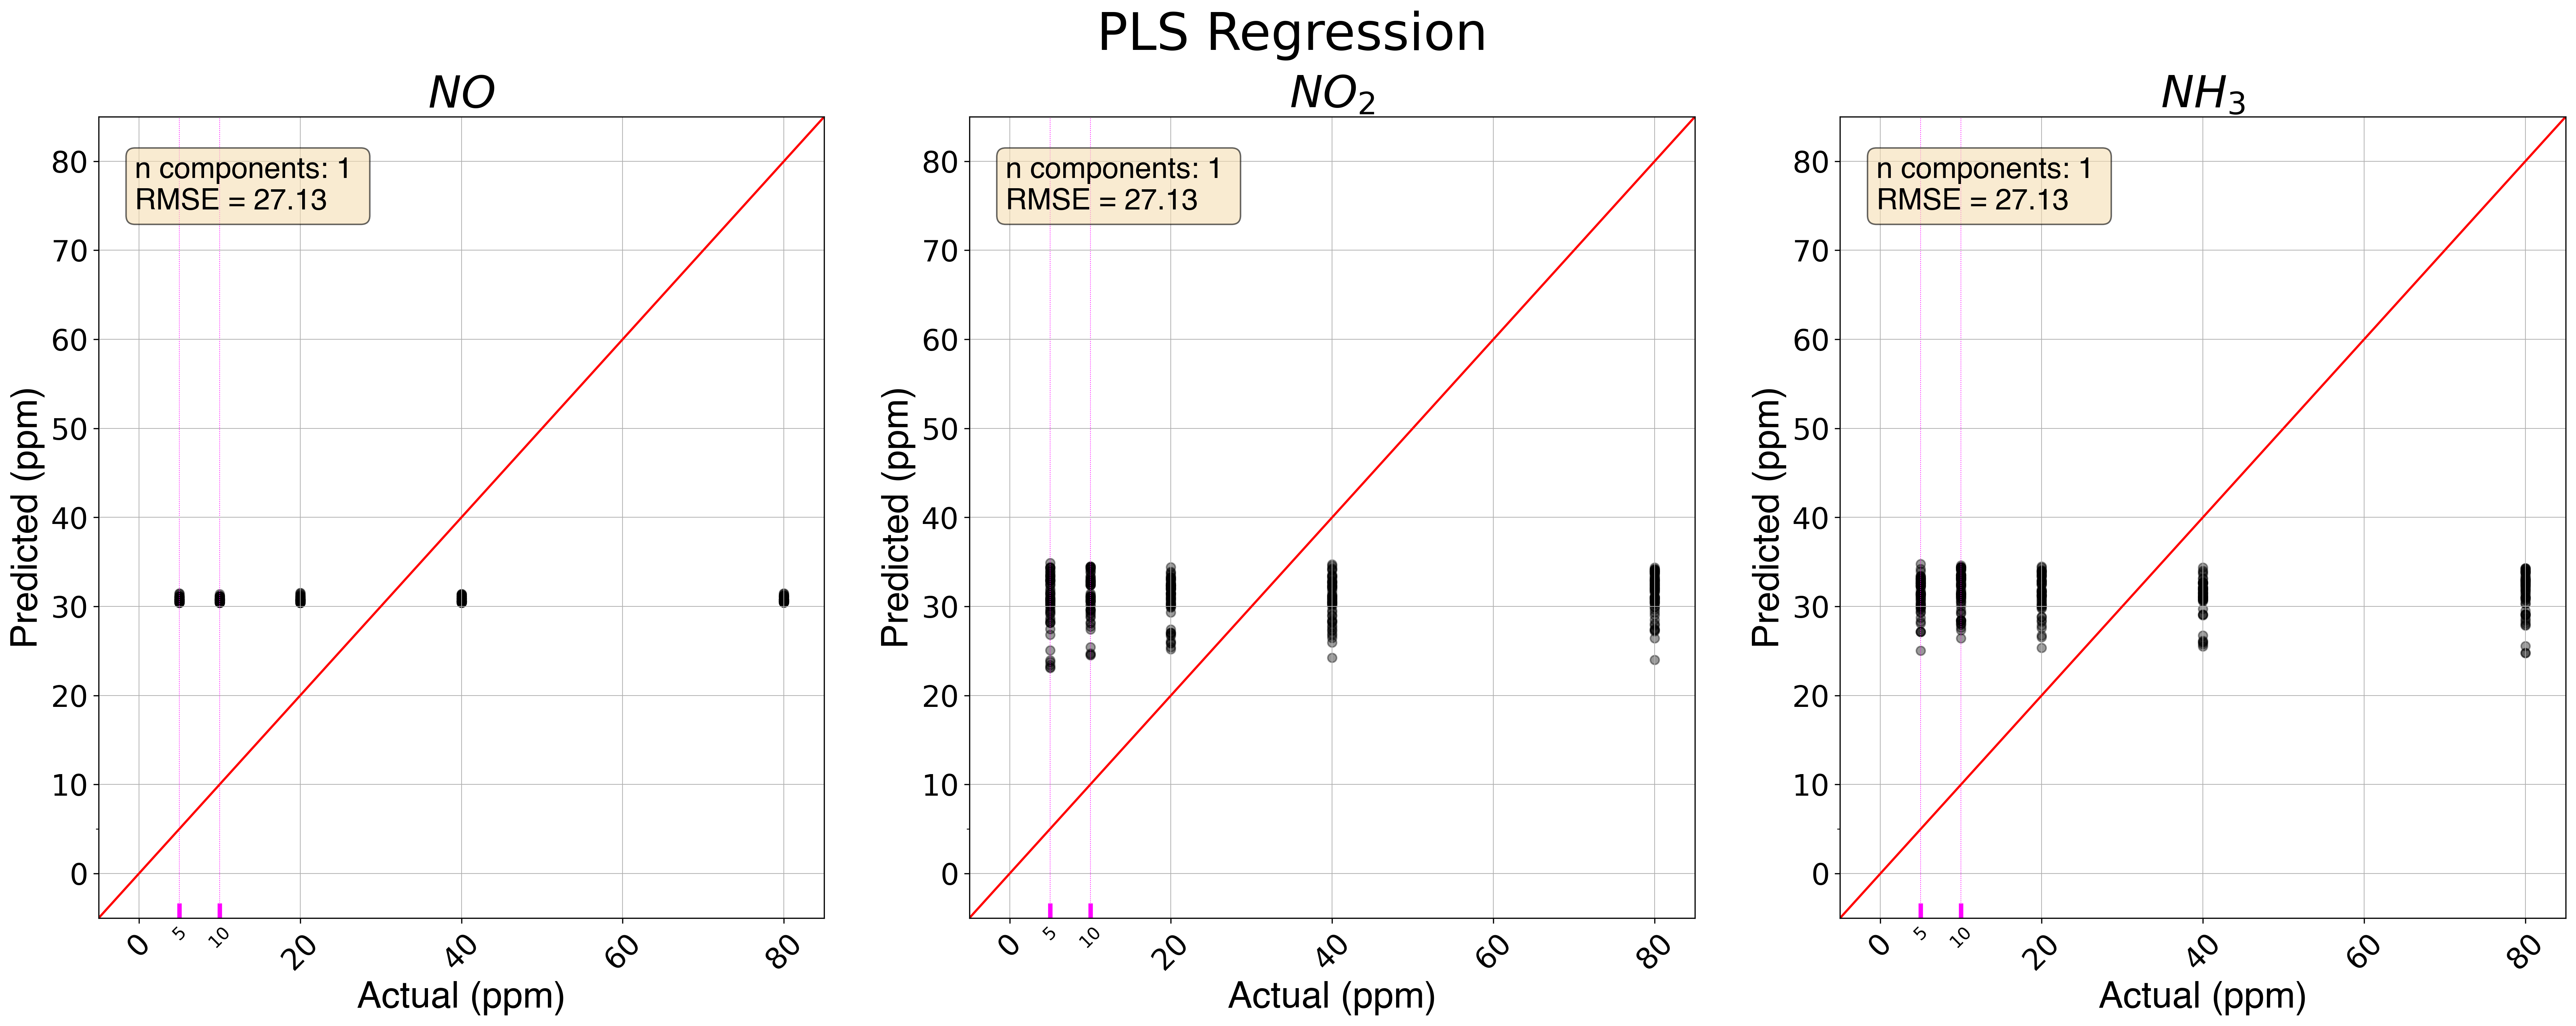
\includegraphics[width=1\textwidth]{../figures/pls-exposures.png}
	\caption{\acrshort{plsr} prediction for individual exposures}
	\label{fig:plsr-exposures}
\end{figure}

\newpage
\subsection{Ridge Regression}

For Ridge regression, the regularization term $\lambda$ was chosen via cross-validation, as shown in Figure~\ref{fig:ridge-cv-exposures}. Additionally, the shrinkage of coefficients can be seen in Figure~\ref{fig:ridge-shrink}. As expected, the coefficients shrink asymptotically towards zero.

\begin{figure}[h]
	\centering
	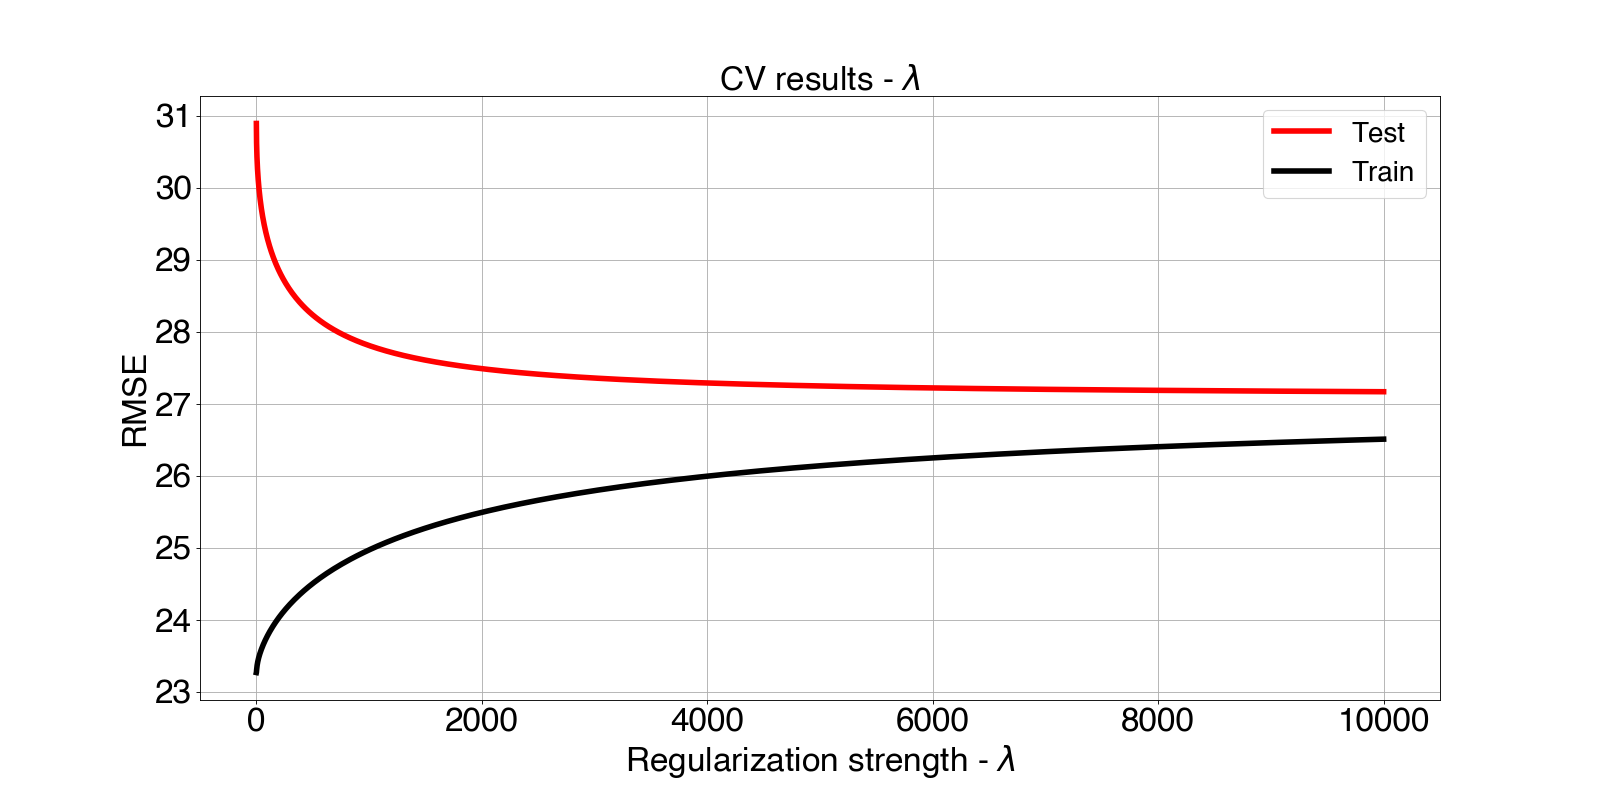
\includegraphics[width=1\textwidth]{../figures/ridge-cv-exposures.png}
	\caption{\acrshort{cv} of shrinkage factor $\lambda$}
	\label{fig:ridge-cv-exposures}
\end{figure}

\begin{figure}[h]
	\centering
	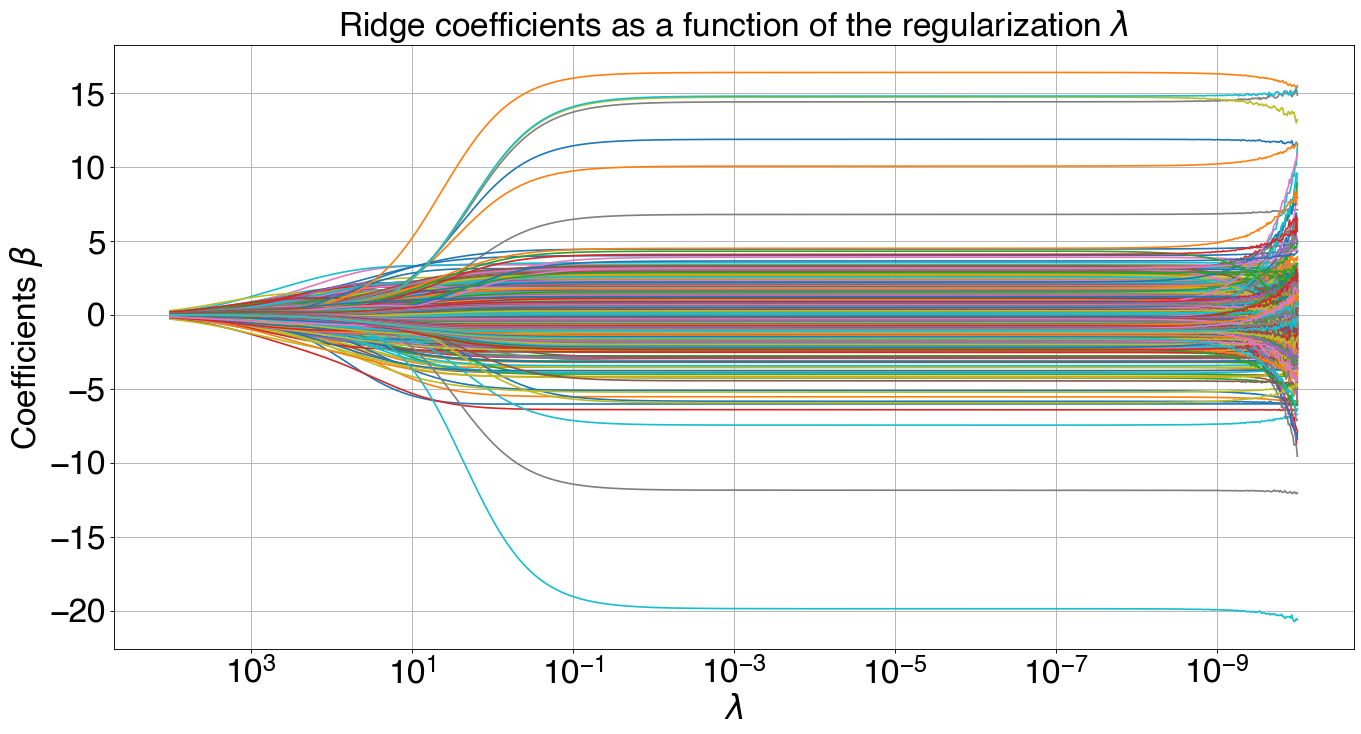
\includegraphics[width=1\textwidth]{../figures/ridge-coefs.png}
	\caption{Shrinkage of ridge coefficients.}
	\label{fig:ridge-shrink}
\end{figure}

Finally, after the choice of $\lambda$, the actual vs. predicted plot is presented if Figure~\ref{fig:ridge-exposures}.

\begin{figure}[h]
	\centering
	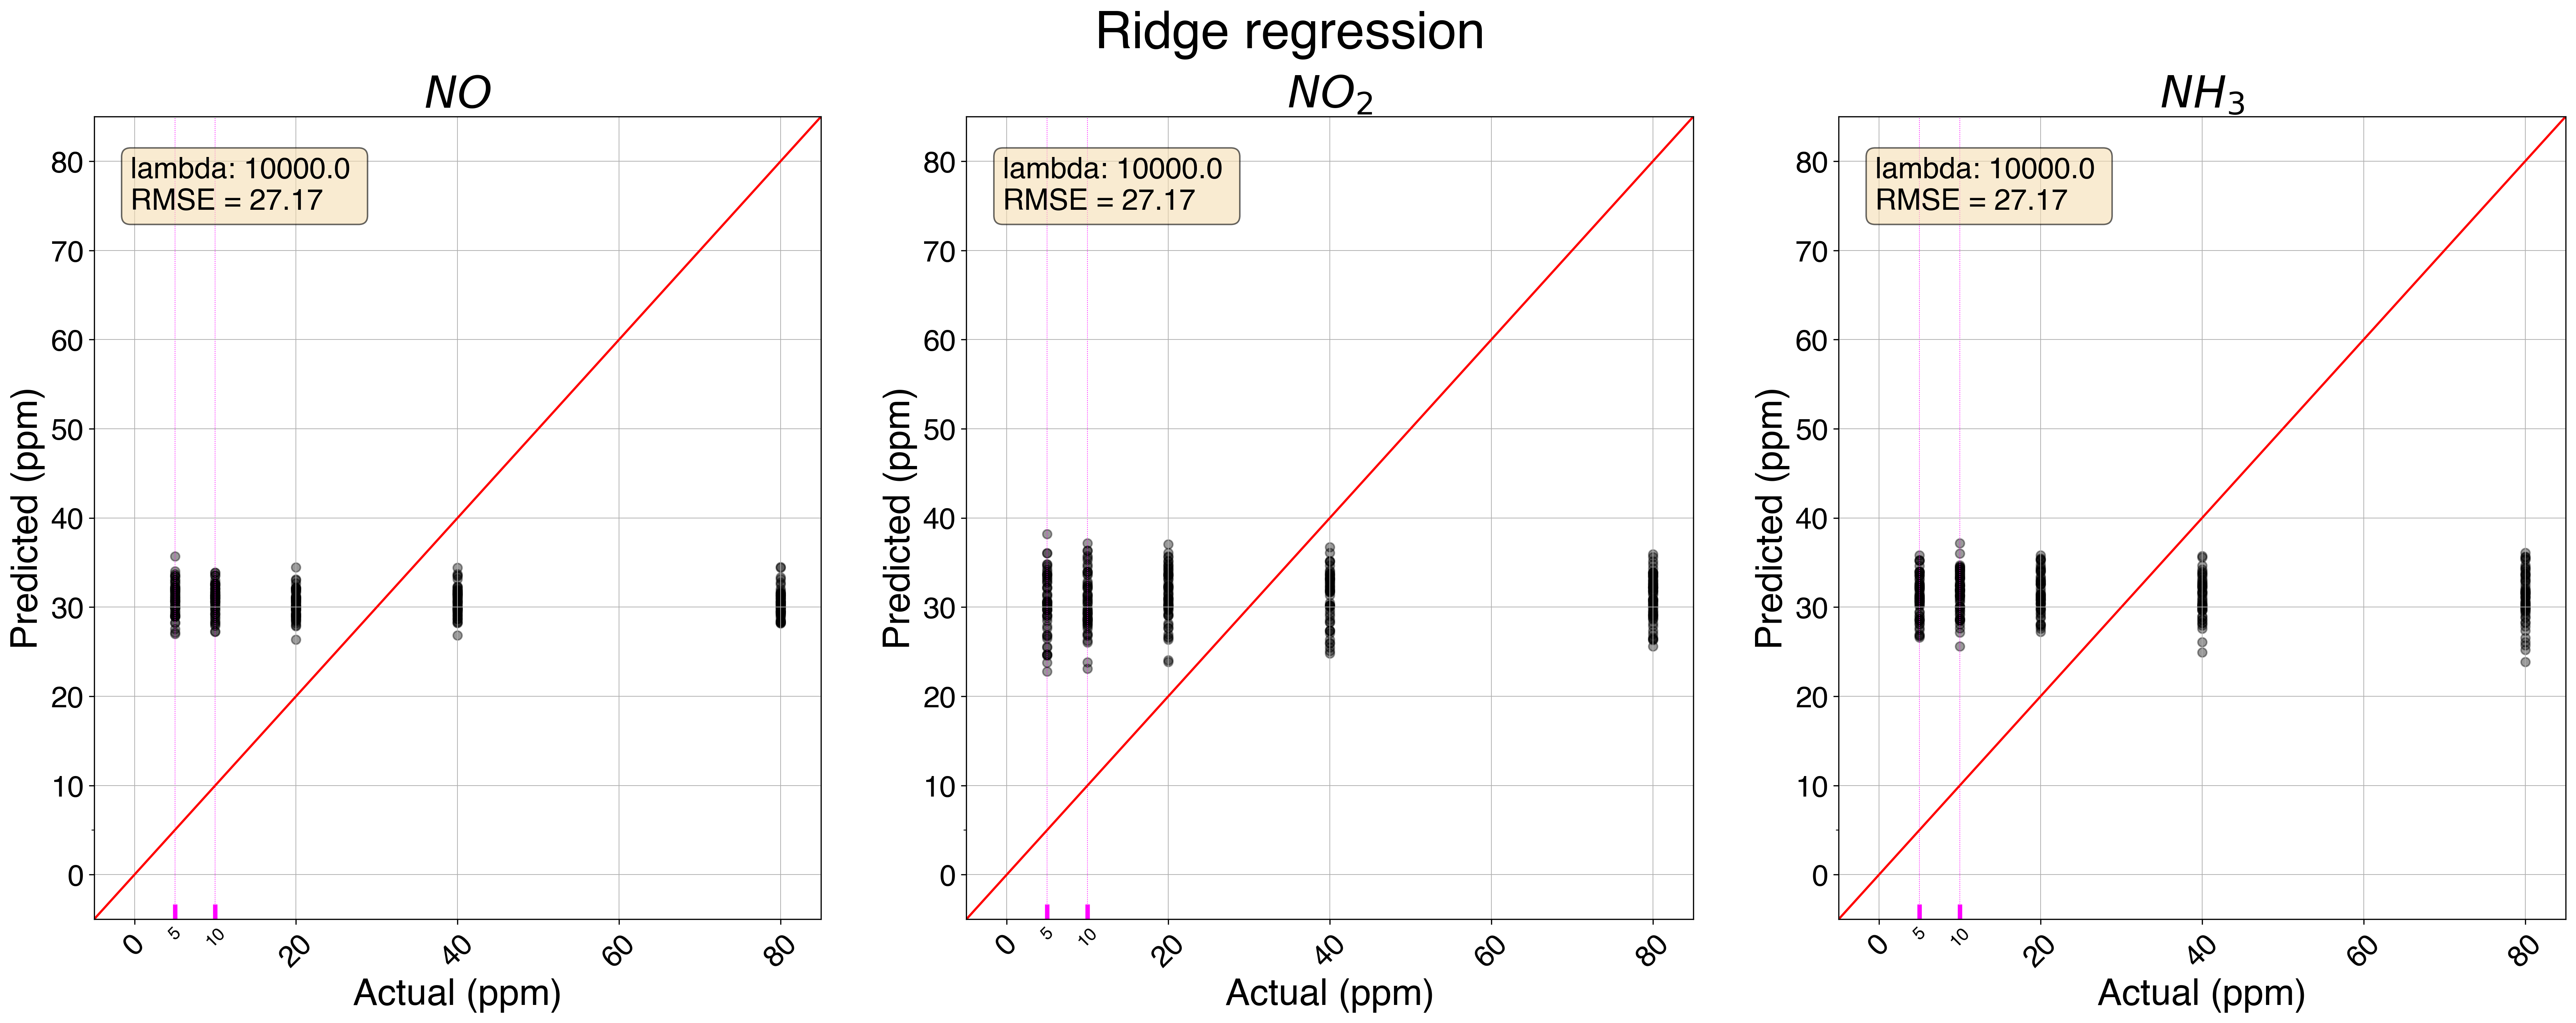
\includegraphics[width=1\textwidth]{../figures/ridge-exposures.png}
	\caption{Ridge prediction for individual exposures}
	\label{fig:ridge-exposures}
\end{figure}


%\section{Averaged exposures} 
%
%\subsection{OLS}
%
%\subsection{PCR}
%
%\subsection{PLSR}
%
%\subsection{Ridge Regression}


%%%%%%%%%%%%%%%%%%%%%%%%%%%%%%%%%%%%%%%%%%%%%%%%%%%%%%%%%%%%%%%%%%%%%%
%%% lorem.tex ends here

%%% Local Variables: 
%%% mode: latex
%%% TeX-master: "demothesis"
%%% End: 
